\newcommand{\versionnumber}{1.2}
\newcommand{\docversion}{
  \renewcommand{\arraystretch}{0.5}
  \setlength{\tabcolsep}{0pt}
  \begin{tabular}[b]{l}
  Versie \versionnumber{}\\
  \today \\
  \end{tabular}
}
\newcommand{\doctitle}{KBS ESA3 \\ Technisch Ontwerp \\ Smart Markers}
\newcommand{\doctitleshort}{TO - Smart Markers}
\newcommand{\docauthor}{
  \renewcommand{\arraystretch}{0.5}
  \begin{tabular}{l l}
  Jerko Lenstra & {\mdseries(S1080179)} \\
  Rick de Bondt & {\mdseries(S1078239)} \\
  Marthijn Tijmes & {\mdseries(S1063534)} \\
  \end{tabular}
}

\newcommand{\doctitlepage}{
  \thispagestyle{empty}

  \parbox[t]{1.0\linewidth}{
    \fontsize{40pt}{60pt}\selectfont
    \doctitle{}
    \fontsize{20pt}{40pt}\selectfont
    \\hbo-ICT, Windesheim
    \\Docent: Gido Hakvoort
  }

  \setlength{\wpYoffset}{-1.8cm}
  \ThisCenterWallPaper{0.75}{technical/windesheim_kadaster.png}
  \vfill

  {
   \docversion{}
   \hspace{185pt}
   \docauthor{}
  }

  \normalcolor{}

  \newpage
}

\providecommand{\doctitle}{Title}
\providecommand{\docauthor}{Author}
\providecommand{\doctype}{scrartcl}
\providecommand{\doctitlepage}{TitlePage}

\documentclass[12pt,a4paper,titlepage,parskip=half]{\doctype}

\usepackage[dutch]{babel}
\usepackage{blindtext}
\usepackage{float}
\usepackage[hidelinks]{hyperref}
\usepackage{graphicx}
\usepackage{listings}
\usepackage{wallpaper}
\usepackage[headsepline,footsepline,manualmark]{scrlayer-scrpage}


% Input and output encoding ---------------------------------------------------
\usepackage{iftex}
\ifPDFTeX
   \usepackage[utf8]{inputenc}
   \usepackage[T1]{fontenc}
   \usepackage{lmodern}
\else
   \ifXeTeX
     \usepackage{xltxtra}
   \else
     \usepackage{luatextra}
   \fi
   \defaultfontfeatures{Ligatures=TeX}
\fi

% Math
\usepackage{amsmath}
\usepackage{amsfonts}
\usepackage{amsthm}
\usepackage{amssymb}
\usepackage{mathtools}

\DeclarePairedDelimiter{\ceil}{\lceil}{\rceil}
\DeclarePairedDelimiter{\floor}{\lfloor}{\rfloor}
\DeclarePairedDelimiter{\bag}{\langle}{\rangle}
\DeclarePairedDelimiter{\set}{\{}{\}}

% Misc
\usepackage[shortlabels]{enumitem}
\usepackage{pgfgantt}

% Bibliography
\usepackage{csquotes}
\usepackage[natbib,style=apa,citestyle=authoryear]{biblatex}
\DeclareLanguageMapping{dutch}{dutch-apa}
\defbibheading{bibliography}[\bibname]{\section{#1}}
\addbibresource{technical/bibliography.bib}

% Display
\usepackage{lastpage}
\usepackage{tabularx}
\setlength{\headheight}{24pt}

\title{\doctitle}
\author{\docauthor}
\date{\today}

\ihead{\upshape{\doctitleshort}}
\ohead{\upshape{\today, v\versionnumber}}
\cfoot{\upshape{\thepage\ /~\pageref{LastPage}}}

\numberwithin{equation}{section}
\numberwithin{figure}{section}
\numberwithin{table}{section}

\usepackage{changepage}

\usepackage{enumitem}
\setitemize{noitemsep,topsep=0pt,parsep=0pt,partopsep=0pt}

% UML
\usepackage[T1]{fontenc}
\usepackage[utf8]{inputenc}
\usepackage{fancyvrb}
% \usetikzlibrary{positioning}
\usetikzlibrary{arrows.meta}
\usepackage{tikz-uml}

%Other settings
\lstset{basicstyle=\ttfamily}

\RedeclareSectionCommand[beforeskip=1\baselineskip,
                         afterskip=.25\baselineskip]{section}

\RedeclareSectionCommand[beforeskip=.25\baselineskip,
                         afterskip=.25\baselineskip]{subsection}

\RedeclareSectionCommand[beforeskip=.25\baselineskip,
                         afterskip=.25\baselineskip]{subsubsection}

\RedeclareSectionCommand[beforeskip=.25\baselineskip,
                         afterskip=.25\baselineskip]{paragraph}

\begin{document}
\doctitlepage{}

\tableofcontents
\thispagestyle{empty}
\newpage

\clearpage
\setcounter{page}{1}
\addtocontents{toc}{\protect\thispagestyle{empty}}

\newpage
\section{Documenthistorie}

\begin{tabularx}{\textwidth}{| l | l | X | l |}
    \hline
    \textbf{Versie} & \textbf{Datum} & \textbf{Verandering} & \textbf{Auteur(s)}
    \\ \hline
    0.1	& 11-jan-2018 & Aanmaken document & Jerko Lenstra \\ \hline
    0.2 & 12-jan-2018 & Toevoegen Product, Proces, Ethische aspecten en Security
     & Marthijn Tijmes \\ \hline

\end{tabularx}


\newpage
\section{Inleiding}
In Nederland is het vanzelfsprekend dat vastgoed geregistreerd is en dat er bekend
is welke gegevens bij dat vastgoed horen. Het Kadaster is verantwoordelijk voor de
vastlegging en verstrekking van vastgoed- en geografische informatie en de rechten
die daarbij horen, zoals eigendom en hypotheek. \citep{KAD_OVER}

Nederland is op gebied van kadastrale registratie vooruitstrevend; in het buitenland
is het niet vanzelfsprekend dat gegevens van vastgoed ergens zijn vastgelegd.
Als gevolg daarvan kan men in deze landen niet aantonen wat hun ontroerend goed is
of wat de waarde daarvan is.

Uit de morele overtuiging dat iedereen recht op eigendom heeft, wat onder andere
opgenomen is in artikel 17 van de Universele Verklaring van de Rechten van
de Mens (UVRM) \citep{UN_UDHR}, wil het Kadaster International deze landen een systeem bieden waarmee
deze eigendommen in kaart gebracht kunnen worden. Dit systeem is recentelijk in
ontwikkeling genomen en het project draagt de naam: \textit{Smart Markers}

\subsection{Aanleiding}
Door het Internet-of-Things keuzesemester van de opleiding hbo-ICT, te Windesheim,
zijn de uitvoerende studenten in aanraking gekomen met dit project. Tijdens het
keuzesemester is er een periode van tien weken waarin studenten aan een project
werken wat in het kader staat van (inter)connectiviteit, duurzaamheid en in het
belang is van de maatschappij.

\subsection{Doel}
Het doel van het project is om ontwikkelingslanden een systeem te bieden dat
een soortgelijke werking heeft als de kadastrale registratie van het Kadaster
in Nederland.

Binnen de scope van tien weken betekent dit het ontwikkelen van een prototype
van een systeem waar locatiegegevens mee kunnen worden verzameld. In hoofdstuk
\ref{sec:opdracht} wordt dit systeem verder uitgediept.


\newpage
\section{Systeemarchitectuur}
Dit hoofdstuk beschrijft de architectuur van het Smart Markers systeem.

\subsection{Architectuur}
De netwerkarchitectuur heeft een stertopologie, waarin de LoRa gateway centraal staat. De GPS-nodes, die om de gateway en over een gebied zijn verspreid, sturen GPS-data naar de gateway. Van één van de GPS-nodes is de positie nauwkeurig opgemeten, deze node functioneert als referentiestation en stuurt GPS-correctiedata naar de gateway. De gateway stuurt deze data door naar een applicatieserver, waar de GPS-data en de GPS-correctiedata worden gebruikt om de GPS-data tot op een meter nauwkeurig te krijgen.

In hoofdstuk \ref{subsec:overzicht} staat een schematisch overzicht van de Smart Markers architectuur.

\subsection{Hardware}
\paragraph{STM32 microcontroller}
Als brein van de Smart Marker is er gekozen voor een \texttt{STM32 NUCLEO-L073RZ development board}, omdat het board:
\begin{itemize}
    \item beschikt over een ARM Cortex M0+ 32 bit processor;
    \item beschikt over voldoende geheugen voor de Smart Marker applicatie;
    \item weinig energie verbruikt;
    \item zich leent voor prototyping;
    \item een veelgebruikte en bekende architectuur heeft;
\end{itemize}

\paragraph{LoRa radio}
De LoRa radio bevindt zich op het RF-LORA-868-SO board. De SX1272 LoRa radio wordt voornamelijk gebruikt voor end-devices, omdat het een half-duplex radio is.
% TODO: Links naar LoRa docs

\paragraph{GPS-modules}
Voor de locatiebepaling worden u-blox EVK-7P GPS-modules gebruikt, omdat Kadaster deze heeft aangeboden voor gebruik tijdens dit project. GPS-modules zijn relatief duur, dus qua budget komt het goed uit dat Kadaster deze modules ter beschikking kan stellen.

Deze GPS-modules worden uitgelezen over de SPI bus, met een maximale snelheid van 1Mb/s. Er zijn twee protocollen voor de representatie van de output data: het UBX protocol voor binaire representatie en het NMEA protocol voor ASCII representatie.
% TODO: Meer onderzoeken. Welke data?

\paragraph{Stroomvoorziening}
Als energiebron gebruiken we twee 18650 cellen, welke extern opgeladen worden.
Om te voorkomen dat deze te ver ontladen worden zal hier een bescherming voor
ingebouwd worden. Voorlopig zullen de cellen extern geladen worden, in een meer
definitieve versie zal het laden geïntegreerd kunnen worden.

\subsection{Software}
Tijdens het project wordt er gebruik gemaakt van softwarepakketten ter ondersteuning. Hieronder staat een korte opsomming van tools en technieken die tijdens het project worden gebruikt:
\begin{itemize}
    \item GNU ARM embedded toolchain;
    \item Makefiles;
    \item ST-Link programmer;
    \item Git;
    \item \LaTeX;
\end{itemize}

\subsection{Communicatie}
Als communicatie techniek is er gekozen voor LoRa, omdat de opdrachtgever met één meting een heel gebied wilt kunnen registreren. De LoRa modulatietechniek leent zich ervoor om in deze use-case gebruikt te worden, vanwege de lange communicatie-afstand en het lage energieverbruik.
% TODO: Bron toevoegen vergelijking communicatie technieken/protocollen

Er is overwogen om een LoRa mesh netwerk op te zetten, echter is er besloten om te kiezen voor een simpelere implementatie, vanwege de korte tijdsduur van het project en een gebrek aan kennis over mesh netwerken. Uit het onderzoek van \citep{AIM_HI_LORA_WMN} is gebleken dat de packet delivery ratio (PDR) in hun labopstelling aanzienlijk betere resultaten had in een mesh netwerk, ten opzichte van een stertopologie.

\subsection{Gegevensopslag}
De verzamelde data uit de meetpunten zal worden opgeslagen in een SQL-database.
Zie ook hoofdstuk \ref{sec:database}.
% TODO: Uitzoeken wat de data throughput is.

\label{subsec:overzicht}
\subsection{Overzicht}
Een totaaloverzicht (afbeelding) van de systeemarchitectuur.


\newpage
\section{Gegevensmodel}
\subsection{Data format}
Het dataformaat van de UBlox is NMEA, NMEA is een standaardprotocol voor het
weergeven van GPS-data. Dit ziet er zo uit: \\
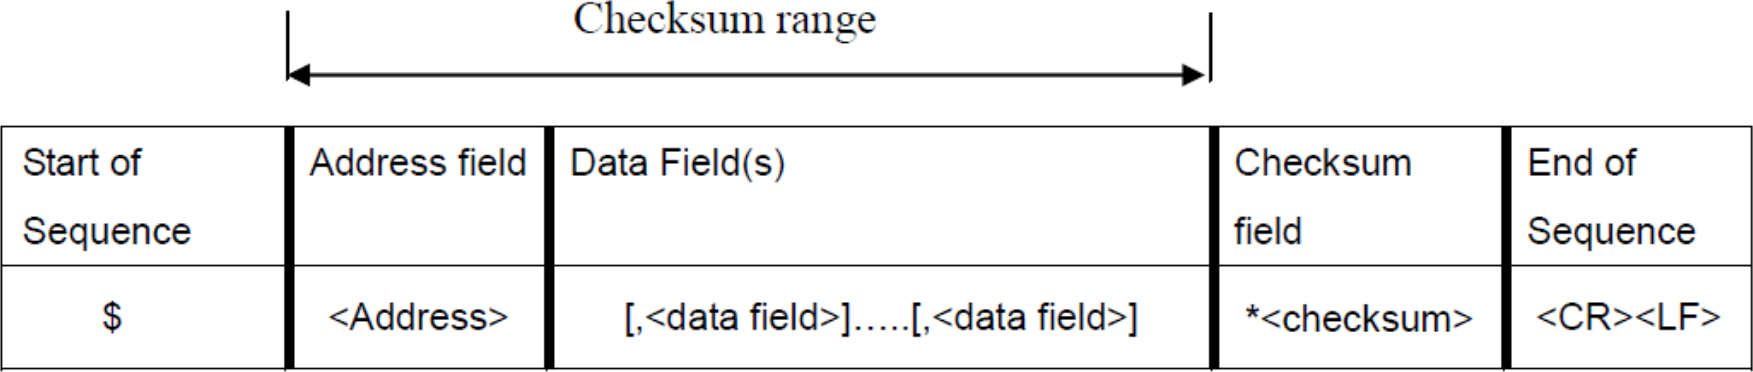
\includegraphics[width=\textwidth]{technical/nmea}
\\Hierbij is het adres veld in het formaat ``aaccc'', waarbij ``aa'' het
Talker ID is en ``ccc'' het soort bericht. Velden zijn gesepareerd met
een ``,''. 
\citep{Navspark}\\\\
Het belangrijkste deel van dit format zijn de GNS-berichten
(GNSS-data). Deze berichten zien er als volgt uit:\\
\texttt{\$GPGNS,091547.00,5114.50897,N,00012.28663,W,AA,10,0.83,111.1,45.6,,,V*71}
\\\\
De velden houden in:
\\\\
\begin{tabularx}{\textwidth}{| l | l | l | l | X |}
    \hline
    \textbf{Veld} & \textbf{Naam} & \textbf{Formaat} & \textbf{Voorbeeld} & \textbf{Beschrijving}          \\ \hline
    0             & xxGNS         & string           & \$GPGNS            & GNS ID (xx = current Talker)   \\ \hline
    1             & Tijd          & hhmmss.ss        & 091547.00          & Tijd (UTC)                     \\ \hline
    2             & Latitude      & ddmm.mmmmm       & 5114.50897         & Latitude (graden en minuten)   \\ \hline
    3             & NS            & character        & N                  & Noord/Zuid                     \\ \hline
    4             & Longtitude    & dddmm.mmmmm      & 00012.28663        & Longtitude (graden en minuten) \\ \hline
    5             & EW            & character        & E                  & Oost/West                      \\ \hline
    6             & posMode       & character        & AA                 & Positionering mode             \\ \hline
    7             & numSV         & numeric          & 10                 & Aantal satellieten             \\ \hline
    8             & HDOP          & numeric          & 0.83               & Horizontal dilution precision  \\ \hline
    9             & alt           & numeric          & 111.1              & Hoogte boven zeeniveau         \\ \hline
    10            & sep           & numeric          & 45.6               & Geoïde separatie               \\ \hline
    11            & diffAge       & numeric          & -                  & Leeftijd correctie             \\ \hline
    12            & diffStation   & numeric          & -                  & ID GPS-correctie station       \\ \hline
    13            & navStatus     & character        & V                  & Navigatie Status               \\ \hline
    14            & cs            & hexadecimal      & *71                & Checksum                       \\ \hline
    15            & <CR><LF>      & character        & -                  & Carriage Return                \\ \hline
\end{tabularx}
\citep[p. 116]{UBlox8}\\
Een ander deel van de data die we mogelijk gaan gebruiken is:
\texttt{\$GPGBS}. \texttt{\$GPGBS} bevat de afwijking van de data bij u-blox
DGPS-toestellen.
\citep[p. 111]{UBlox8}

De uiteindelijke data die we gaan gebruiken is:
ID, Tijd (UTC), Latitude, Longtitude en Altitude

Voor het referentiestation komt hier nog bij:
error Latitude, error Longtitude en error Altitude

\subsection{Database}
\label{sec:database}

De verstuurde data zal worden bijgehouden in een SQL-database. Tijdens het testen
zal dit op een extern gehoste server zijn.
Wanneer er een eigen LoRa gateway met de markers gebruikt wordt zal deze database
een lokaal, offline, systeem zijn. De data zal dan naar een centrale database
worden verstuurd wanneer er een goede internetverbinding is.

De tabel met de meetpunten zal de volgende kolommen bevatten:
\begin{itemize}
    \item Meetpunt ID
    \item Marker nummer
    \item Latitude
    \item Longitude
    \item Tijdstip van registratie
\end{itemize}

Verder zal er een tabel zijn met de percelen, deze bevat de kolommen:
\begin{itemize}
    \item Perceel ID
    \item Perceelnummer
\end{itemize}

Om de percelen en meetpunten aan elkaar te koppelen zal er een koppeltabel komen:
\begin{itemize}
    \item Perceel ID
    \item Volgnummer
    \item Meetpunt ID
\end{itemize}

\subsection{Bestanden}
\subsubsection{Code}


\newpage
\section{Klassendiagram}
\subsection{Overzicht}
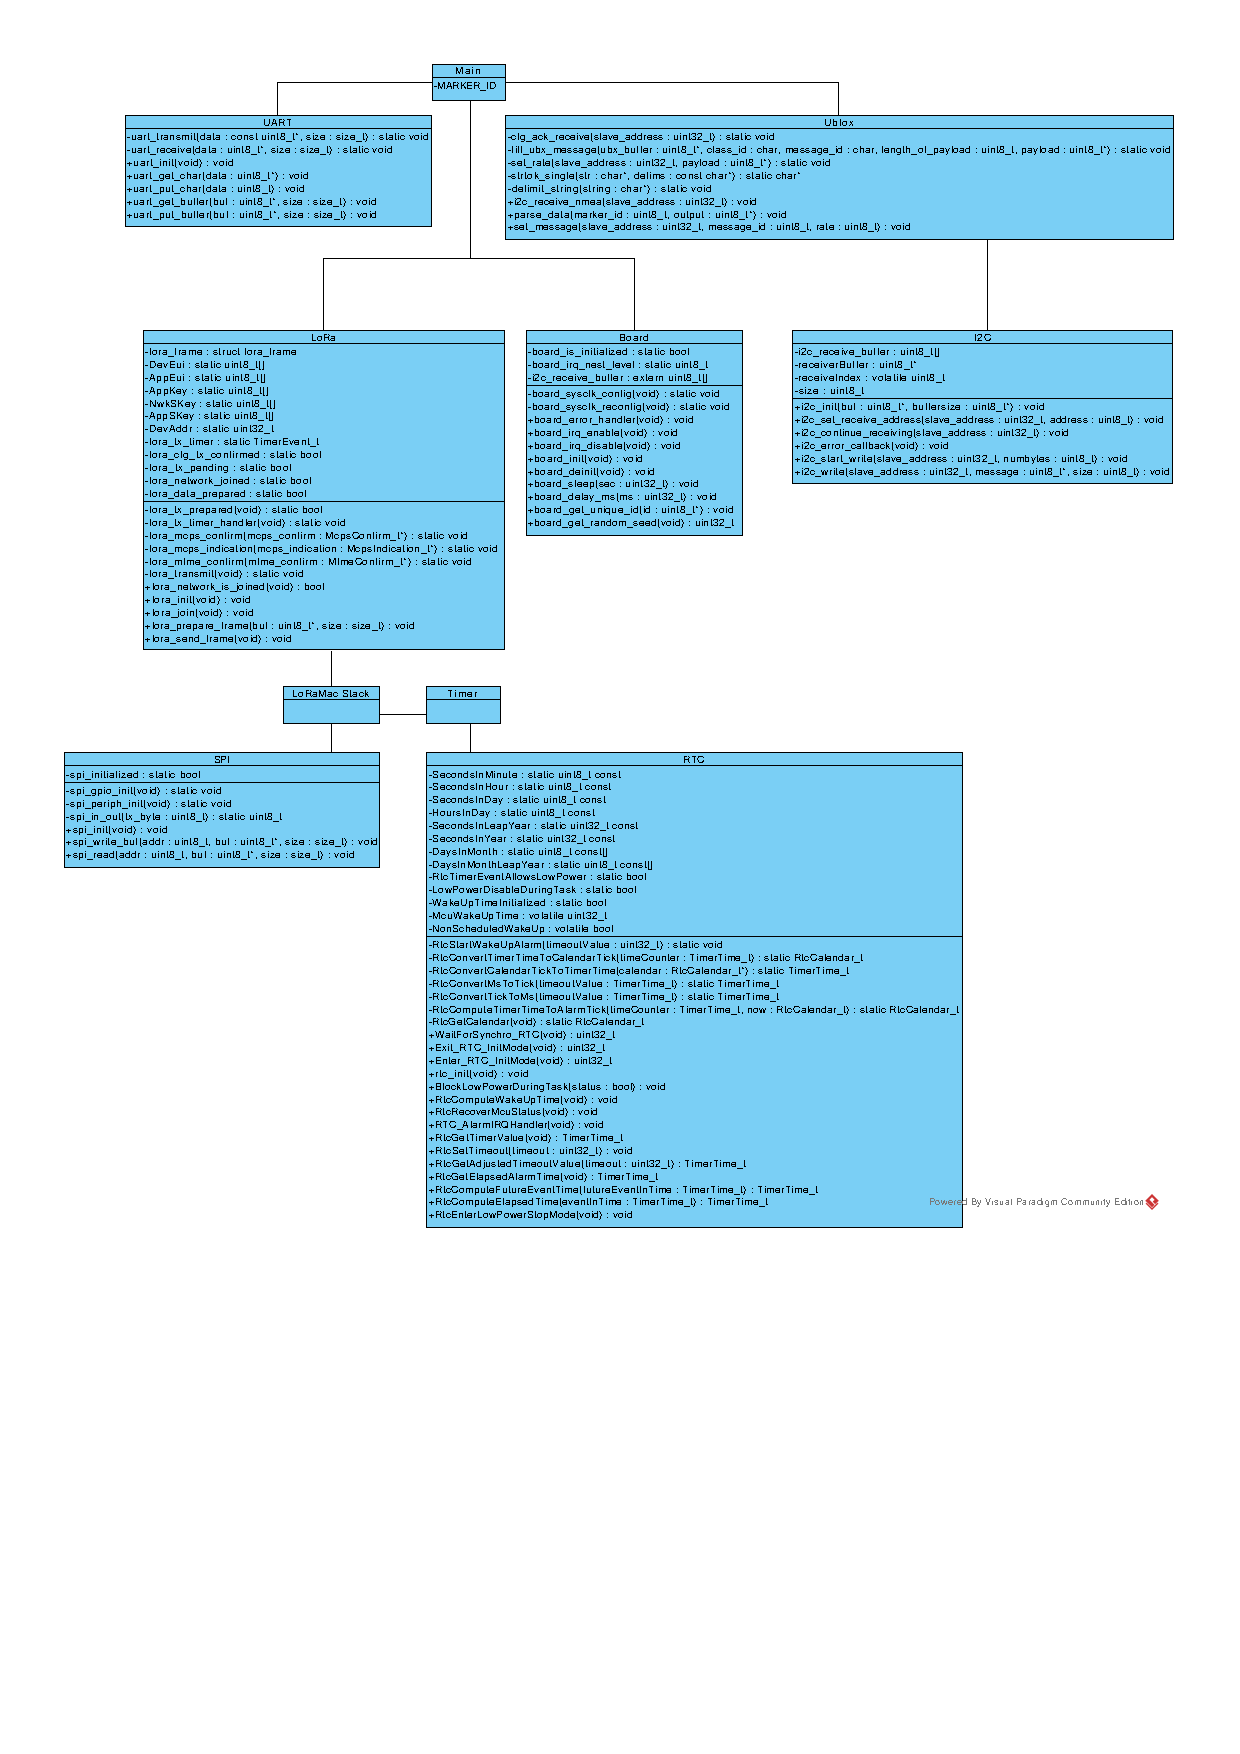
\includegraphics[width=0.9\textwidth]{technical/class_diagram.pdf}

\subsection{Eigen code}
\subsubsection{Main}
Dit is het entry point van de C code. Deze file bevat alleen de code die van belang
is voor de user, dat betekent dat de code zo simpel mogelijk is gehouden.

De user applicatie kijkt of de Smart Marker met een LoRaWAN netwerk verbonden is
en, zo ja, verstuurt dan de gemeten GPS-data over het netwerk. Wanneer er nog
geen verbinding is blijft hij proberen om connectie te maken.

\subsubsection{Board}
In dit interface staan de board ondersteunende functies (b.v. het uitschakelen van
interrupts) die door heel de programmatuur worden gebruikt.

De user applicatie zal niet werken als \texttt{board\_init()} niet als eerste
functie wordt aangeroepen.

\subsubsection{UART}
Deze driver wordt in de user applicatie doorgaans niet gebruikt, maar deze is
ontwikkeld om het debuggen makkelijker te maken.

\subsubsection{I2C}
Het I2C interface is ontwikkeld om de GPS-module uit te kunnen lezen. De inkomende
data wordt in een buffer opgeslagen, die in het \texttt{Ublox} interface wordt
uitgelezen.

\subsubsection{SPI}
Het SPI interface is geschreven om de LoRa radio registers te programmeren. Het
is ook te gebruiken om de GPS-module uit te lezen, echter is dat niet gebruikt in
deze applicatie.

\subsubsection{RTC}
De Real-Time Clock wordt gebruikt in het \texttt{Timer} interface, wat door Semtech
is ontwikkeld. De RTC stelt een interrupt in, zodat het board wakker gemaakt kan
worden op de gewenste datum of het gewenste tijdstip.

\subsubsection{LoRa}
Dit interface dient als laag tussen de user applicatie en de \texttt{LoRaMac} ofwel
de LoRaWAN netwerk stack. Het is geschreven om de werking en instellingen van LoRaWAN
te abstraheren voor de gebruiker. Zo is het makkelijker om een andere user applicatie
te schrijven.

\subsubsection{Ublox}
Het Ublox interface is geschreven specifiek voor de GPS-module die gebruikt is
tijdens dit project. Het staat de gebruiker toe om instellingen te veranderen in
de module, zodat b.v. het krijgen van een GPS-fix minder lang duurt, of om de
frequentie van berichten in te stellen.

\subsection{Gebruikte code}
Omdat het draait om de code die de studenten hebben geproduceerd, is gebruikte
code zoveel mogelijk buiten het klassendiagram gehouden.

\subsubsection{LoRaMac van Semtech}
Semtech, de producent van de LoRa chips, heeft in samenwerking met wat kleinere
bedrijven een implementatie gemaakt die overeenkomen met de LoRaWAN specificaties.
Dit project, genaamd LoRaMac, is gebruikt als basis voor de Smart Marker LoRa
implementatie.

Deze code staat in de directory: \texttt{code/smart\_marker/lora}.

\subsubsection{STM32L0xx CMSIS / low-layer drivers}
STMicroelectronics, de producent van het development board waarmee gewerkt is,
heeft een aantal board ondersteunende soft-/firmware pakketten die het makkelijker
maken om te ontwikkelen met de hardware.

Deze code staan in de directories:
\begin{itemize}
    \item \texttt{code/smart\_marker/bsp/cmsis}
    \item \texttt{code/smart\_marker/bsp/stm32l0xx\_hal}
\end{itemize}

\newpage
\section{Activity Diagram}
Het onderstaande diagram geeft een globale weergave van de werking van de Smart
Marker. Er is voor gekozen om het diagram minimalistisch te houden, aangezien
de volledige werking van het project niet overzichtelijk wordt door het in een
activity diagram te tonen.

% \vspace*{2cm}
\begin{center}
{
    \large
    \begin{tikzpicture}[>=stealth,
        every node/.style={
            shape=rectangle,
            draw,
            rounded corners,
            line width=1pt},
                        ]
    % create the nodes
    \node (n0) [shape=circle, fill=black] {};
    \node (n1) [below = of n0] {Board: initialise peripherals and clocks};
    \node (n2) [below = of n1] {LoRa: initialise network stack};
    \node (n3) [below = of n2] {GPS: initialise module};
    \node (n4) [below = of n3] {GPS: get location fix};
    \node (n5) [below = of n4] {GPS: update and parse location data};
    \node (n6) [below = of n5] {LoRa: is network joined?};
    \coordinate[left = 2 of n6] (c0);
    \coordinate[right = 2 of n6] (c1);
    \node (n7) [below = 2 of c0] {LoRa: join network};
    \node (n8) [below = 1.5 of c1] {LoRa: prepare frame};
    \coordinate[right = 2 of n8] (c2);
    \node (n9) [below = of n8] {LoRa: send frame};
    \coordinate[below = 6 of n5] (c3);
    \node (n10) [below = of c3] {Board: sleep};
    % connect the nodes
    \draw[line width=1pt,-{Latex[length=3mm]}] (n0) to[out=270,in=90] (n1);
    \draw[line width=1pt,-{Latex[length=3mm]}] (n1) to[out=270,in=90] (n2);
    \draw[line width=1pt,-{Latex[length=3mm]}] (n2) to[out=270,in=90] (n3);
    \draw[line width=1pt,-{Latex[length=3mm]}] (n3) to[out=270,in=90] (n4);
    \draw[line width=1pt,-{Latex[length=3mm]}] (n4) to[out=270,in=90] (n5);
    \draw[line width=1pt,-{Latex[length=3mm]}] (n5) to[out=270,in=90] (n6);
    \draw[line width=1pt,-{Latex[length=3mm]}] (n6) to[out=180,in=90]
        node[draw=none,fill=none,pos=.2,above] {No} (n7);
    \draw[line width=1pt,-{Latex[length=3mm]}] (n6) to[out=0,in=90]
        node[draw=none,fill=none,pos=.2,above] {Yes} (n8);
    \draw[line width=1pt,-{Latex[length=3mm]}] (n7) to[out=270,in=90] (n10);
    \draw[line width=1pt,-{Latex[length=3mm]}] (n8) to[out=270,in=90] (n9);
    \draw[line width=1pt,-{Latex[length=3mm]}] (n9) to[out=180,in=90] (n10);
    \draw[line width=1pt] (n10) to[out=0,in=270]
        node[draw=none,fill=none,pos=.3,below,yshift=-10pt]
        {[Current time > Sleep time]} (c2);
    \draw[line width=1pt,-{Latex[length=3mm]}] (c2) to[out=90,in=0] (n4);
    \end{tikzpicture}
}
\end{center}

\newpage
\section{Gebruikersinterface}
\subsection{Dataweergave}
Voor het weergeven van de meetpunten is gekozen voor een JavaScript plugin van Google.
Op deze manier laat zich eenvoudig een Google Maps kaart tonen op de website waarop we de
meetpunten en percelen eenvoudig kunnen tonen.

Het importeren van de meetpunten wordt gedaan door de meetpunten te exporteren naar een
KML-bestand, welke de coordinaten en overige gegevens van de punten bevat. Deze worden
door een PHP-script uit de SQL-database gehaald en vervolgens geprint in het KML-bestand.
Deze worden vervolgens als pins binnen Google Maps getoond. Om te voorkomen dat er een
door Google gecachte versie van het KML-bestand getoond wordt, wordt de time() functie van
php gebruikt om bij elke aanroep een nieuwe URL te creëren.

Door op een pin te klikken wordt de bijbehorende informatie getoond, samen met een 'Voeg
aan perceel toe' button, om de geselecteerde marker toe te voegen aan een nieuw perceel.

Op de achtergrond maakt een Javascript functie hier een array van, welke samen met de
ingevoerde naam verzonden wordt naar de server.
Wanneer er een perceel verzonden wordt, maakt de database hier eerst een perceel ID voor
aan, vervolgens worden alle meetpunten in de array met het nieuwe perceel ID toevevoegd
aan de link\_table.

De percelen worden ook verwerkt tot een KML-bestand. Hierin wordt per perceel een nieuwe
polygoon aangemaakt, waarin op volgorde van aanklikken de meetpunten als hoekpunten
toegevoegd worden. Dit wordt gedaan door een automatisch verhogend ID veld te hebben in de
link\_table en hierop ook weer te sorteren.

Wanneer op een polygoon geklikt wordt, toont de website enige informatie over dit perceel.
Op dit moment de naam en het tijdstip van creëren, maar dit is eenvoudig aan te passen naar
meer informatie indien gewenst.


\subsection{Advies}
De Google Maps plugin is afhankelijk van internet, dat wil zeggen dat er een actieve
verbinding moet zijn om het kaartmateriaal te downloaden. Dit kan in het veld een
probleem zijn.


\newpage
\printbibliography

\end{document}
